\documentclass[12pt,a4paper]{report}
\usepackage[utf8]{inputenc}
\usepackage[T1]{fontenc}
\usepackage[czech]{babel}
\usepackage{graphicx}
\graphicspath{{./assets/}}

\usepackage{url}
\author{Michal Žáček}
\title{{\Huge Blender pro Smrtelníky}\\ {\Large Příručka k Blenderu v2.8} \\ {\large Ročníková Práce}}
\date{2019/20}

\pagestyle{headings}

\begin{document}
		\maketitle
	\pagebreak
	{
		\centering
	{\Huge MENSA GYMNÁZIUM, o.p.s.} \\
	{\Large ROČNÍKOVÁ PRÁCE} \\
	
	\textit{Strukturalizovaná příručka k 3D Grafickému programu Blender}
	
	{\large Obor: Počítačová Grafika
\\
		Autor: Michal Žáček \\}
	}
	\begin{itemize}
	\item[] Třída: Septima
	\item[] Školní rok: 2019/20
	\item[] Vedoucí práce: Hana Šromová
	\item[] Oponent/Konzultant: Dominika Lippertová
	\item[] Rozsah práce (s.):
	\begin{itemize}
		\item[] celkový (včetně této strany, vyjma titulní): 
		\item[] vlastní text:
		\item[] vědecký aparát (poznámky, bibliografie aj.):
	\end{itemize}
	\item[] Formát elektronické podoby práce: PDF
	\end{itemize}
\begin{abstract}
	\paragraph{Anotace} Tato práce se snaží namísto obvyklých internetových tutoriálů přiblížit. Blender jako software systematicky a s mnohými okolními znalostmi,
	které jsou potřebné k jeho plnému využití. Snažím se předat znalosti
	tak, aby čtenář pochopil logiku, na které stojí úkony, které provádí a
	byl schopen vyvozovat z nich závěry, pomáhající při dalším rozvíjení a
	používání programu.
	\paragraph{Klíčová Slova} 3D Grafika, Blender, Příručka, Výukový Materiál
	\paragraph{Anotace (AJ)} This work tries instead of the usual internet tutorials to approach
	Blender as a software systematically and with many surrounding
	knowledge that is needed to fully use it. I try to pass on the knowledge
	in such a way, that the reader understands the underlying principles on
	which the actions he performs stand and so that he may later be able
	to draw conclusions from them, helping to use and develop their use of
	the program.
	\paragraph{Klíčová Slova (AJ)} 3D Graphics, Blender, Handbook, Educational Material
\end{abstract}
	\pagebreak
	\tableofcontents
	\pagebreak
	
	\chapter{Předmluva}
	\section{Informace o Dokumentu - Cílová Skupina, Styl a Záměr}
	Psáno pro Blender 2.8. Tento dokument má zahrnovat základní znalosti
	potřebné k rozumné práci ve 3D grafických programech se zaměřením na
	Blender.
	Je důležité vědět, že cílem této práce je seznámit čtenáře s Blenderem do
	takové míry, aby byl schopen sám začít prozkoumávat tento rozsáhlý
	program. Mnohé části jsou přeskočeny nebo vysvětleny povrchně za
	účelem nezahltit čtenáře.
	Účelem je vysvětlit, jak funguje Blender spíše v jeho principech a s
	některými nuancemi, které mohou nováčkům dělat problém. Je mnoho
	lidí, kteří se již do modelování v Blenderu chtěli pustit, ale poté, co si našli
	na internetu nějaké tutoriály, stejně nevěděli, co dělali, protože jenom
	slepě sledovali tutoriál bez hlubšího pochopení. Pochopení problematiky,
	schopnost stavby na předešlých znalostech a zkoušení si sám nových
	věcí, je stav, který je právě záměrem této práce.
	\section{Kde všude se používá}
	„Používám Blender protože je silný, ne protože je zdarma“, řekl Max
	Puliero v rozhovoru s CGCookie.com v roce 2017. \cite{cgcookiePuliero} Od té
	doby, především během několika posledních pár let, se Blender přeměnil
	z komerčně téměř nepoužívaného programu v extrémně výkonný kus
	softwaru, který by mohl konkurovat mnohým placeným alternativám.
	Příklady, kde Blender byl použit:
	Max Puliero uvedl, že při práci na hře Dark Souls III, používal na design
	postav Blender, přestože jeho studio standartně užívalo jiné programy.
	\cite{cgcookiePuliero} Ubisoft Animation Studio má v průběhu roku 2020
	adoptovat Blender jako svůj hlavní software. \cite{ubisoft-news-BlenderDevFund} Unity Game
	Engine nativně podporuje [.blend] soubory.
	Již dlouho existovaly filmy tvořené pomocí Blenderu, ale Next Gen (2018)
	od Netflix je jeden z prvních komerčních filmů, které byly skutečně
	animovány čistě v Blenderu (Veldhuizen, 2018). Pokud nebereme celý
	film, ale stačí využití, pak ve filmu Warcraft (2016) byl narychlo přidán
	Murloc s jeho pomocí. (Failes, 2016)Pokud se zajímáte spíše o vesmír, NASA vydala některé z jejích modelů
	v [.blend] formátu. Dokonce projekt Experience Curiosity nějakou dobu
	běhal na Blender Enginu, dokud nebyl zrušen.
	Takže jak sami vidíte, není toho málo.
	\begin{figure}
		\centering
		\includegraphics[scale=0.25]{next-gen.jpg}
		\caption{Next Gen Film \cite{netflix-nextgen}}
		\label{pic:netflix-nextgen}
	\end{figure}
	
	\section{Blender Foundation - Trocha Historie \\ \cite{wikiBlender}}
	\begin{figure}[h]
		\centering
		\includegraphics[scale=0.3]{Ton-Roosendaal.jpg}
		\caption{Ton Roosednaal \cite{ton-roosendaal}}
		\label{pic:ton-roosendaal}
	\end{figure}
	
	\begin{figure}[h]
		\centering
		\includegraphics[scale=0.45]{man03.jpg}
		\caption{Blender circa 2002 \cite{blender-man}}
		\label{pic:blender-man}
	\end{figure}
	NeoGeo bylo dánské animační studio, které roku 1994 začalo vytvářet
	Blender pro firemní použití. Hlavním autorem byl Ton Roosendaal –
	tehdejší spolumajitel firmy. V roce 1995 už měli funkční verzi 1.0 a 1.
	ledna 1998 byl jejich program vydán jako freeware – volně dostupný na
	internetu. Ještě ten samý rok byla firma NeoGeo zanikla a Roosendaal
	založil svoji vlastní firmu Not a Number Technologies (NaN), za účelem
	dále rozvíjet projekt Blender. NaN roku 2002 zkrachovala a Roosendaal
	ještě téhož roku založil neziskovou organizaci Blender Foundation.
	Blender Foundation se během následujících let pokoušel udělat Blender
	Open-Source (prozatím byl Blender pouze volně dostupný jako celý
	program, open-source znamená, že bude i volně upravitelný a bude na
	něm moct pracovat kdokoli). Roosendaal vybral svůj cíl 100 000 euro od
	lidí a dosáhl svého cíle. Dodnes je Blender vyvíjen hlavně jeho komunitou
	a čtyřmi programátory zaměstnanými u Blender Foundation.
	
	\section{Blender není jen na 3D modelaci}
	Ačkoli začal svůj život jako animační program, vyvíjen pro potřeby
	animace, rozsáhlá komunita mu přidala množství různých dalších funkcí.
	Dnes zvládá editovat video, zvuk, zvládá sledovat objekty na kameře a
	nedávno se objevily i fotogrammetrické pluginy. Rozšířila se také podpora
	jiných programů. Není vzácné, aby herní engine měl podporu pro
	proprietární [.blend] soubory nebo podporoval přímé napojení pomocí
	pluginů.
	
	\section{Pluginy}
	Roztroušenost vývoje donutila Blender využívat tzv. pluginy. Plugin je
	funkce programu taková, že není brána jako součástí jeho jádra, ale bere
	se jako jeho rozšíření. Lze jej například i vypnout nebo stáhnout z
	internetu. Příkladem je třeba podpora dalších formátů, předpřipravené
	nové objekty a zjednodušený přístup k některým nastavením. Takových
	pluginů je obrovské množství a dají se doinstalovat do Blenderu podle
	potřeby. On sám už nějaké obsahuje, a i když jsou některé v základu
	vypnuty, není kolikrát potřeba je stahovat a lze je pouze zapnout v
	nastavení.
	
	\chapter{Interface}
	Blender se s pomocí své rozmanité funkčnosti snaží poskytnout co nejvíce
	možností a do toho je musí udržet přístupné a přehledné. K tomuto
	využívá systém oken, o kterém si nyní něco můžeme říct.
	Když poprvé spustíte Blender, tak vypadá následovně.
	
	\begin{figure}[h]
		\centering
		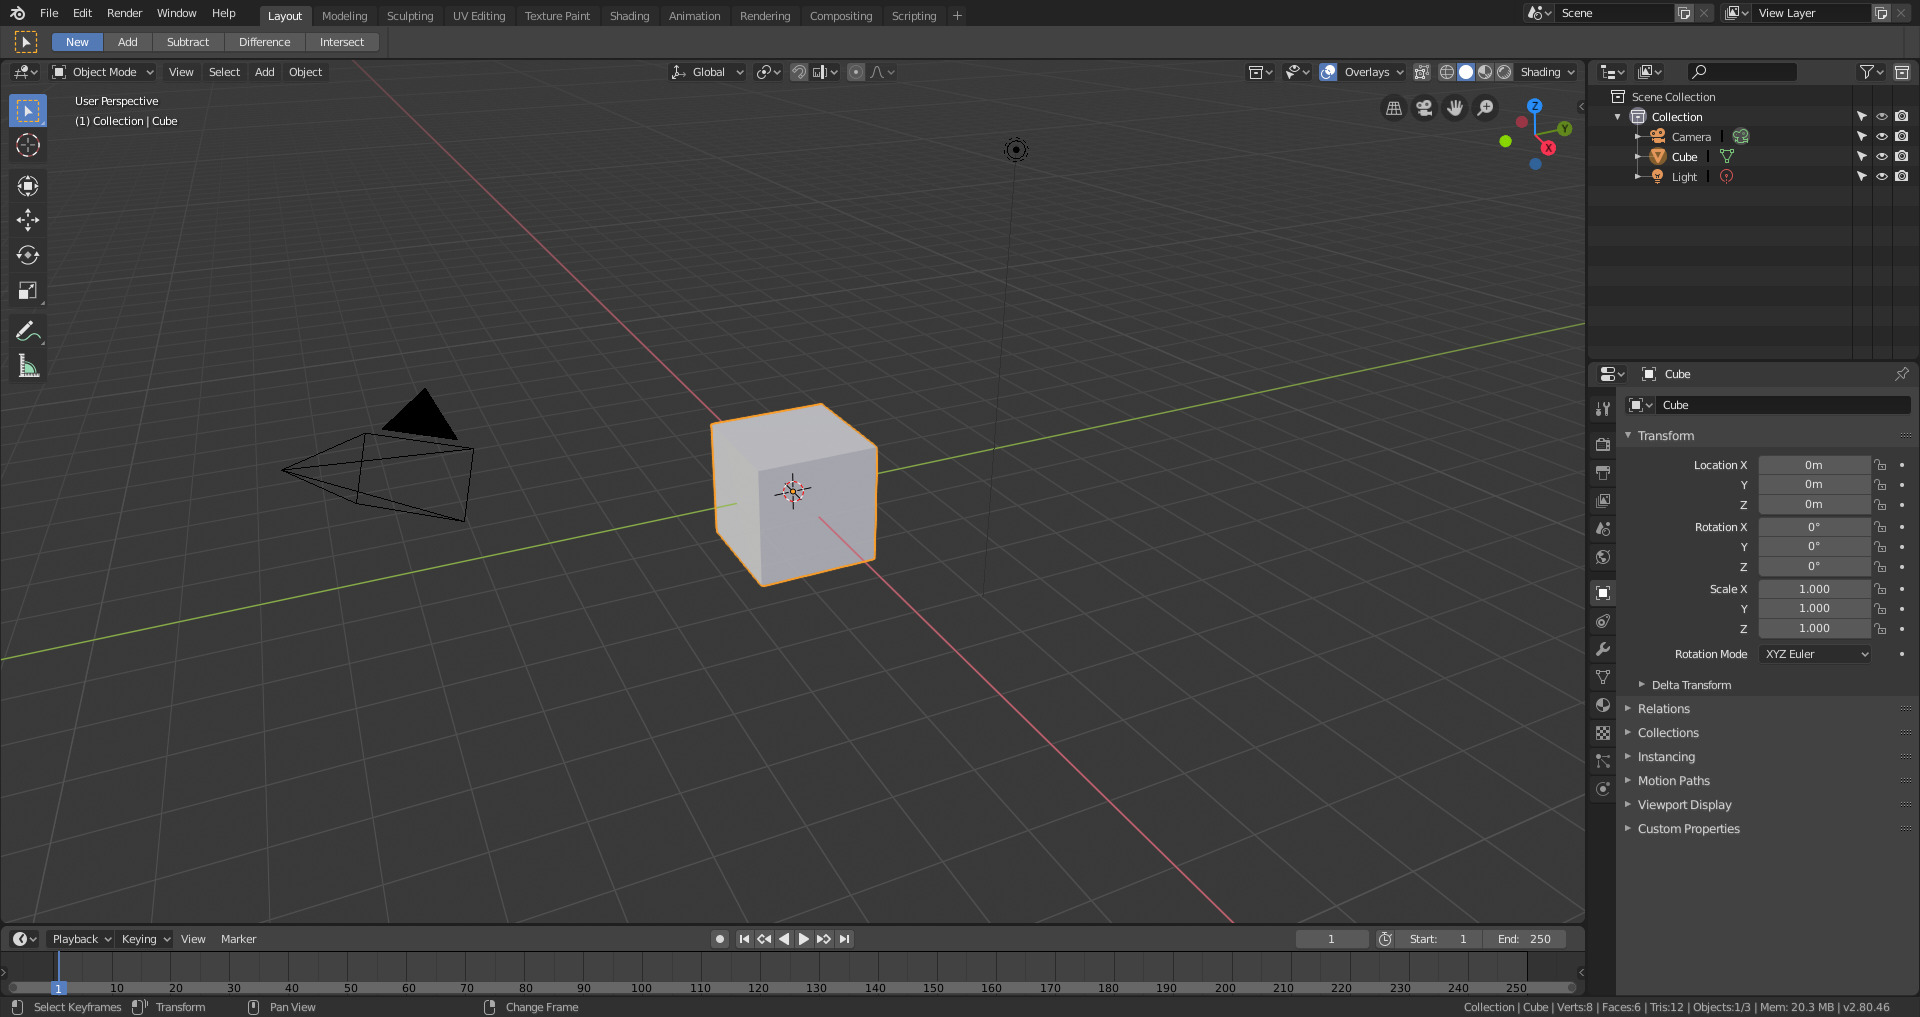
\includegraphics[scale=0.25]{UI/UI-1.png}
		\caption{Po spuštění}
		\label{pic:startup-1}
	\end{figure}

	Nejlépe je si přirovnat systém Blender k oknům u Vašeho počítače. Tak,
	jak máte na počítači otevřena mnohá okna vedle sebe (např.: prohlížeč,
	Word, mail atd.), stejně tak je to u Blenderu. Blender jako program má
	nespočet různých funkcí, které by byly absolutně nepochopitelné, kdyby
	byly ukázány všechny najednou. Proto jsou nástroje uvedeny do
	souvisejících oken, kdy každé z nich má sloužit k jednomu účelu -například okno pro umístění objektů do scény, okno pro jejich nastavení,
	okno pro editaci videa, okno pro práci s texturami atd.
	
	\begin{figure}[h]
		\centering
		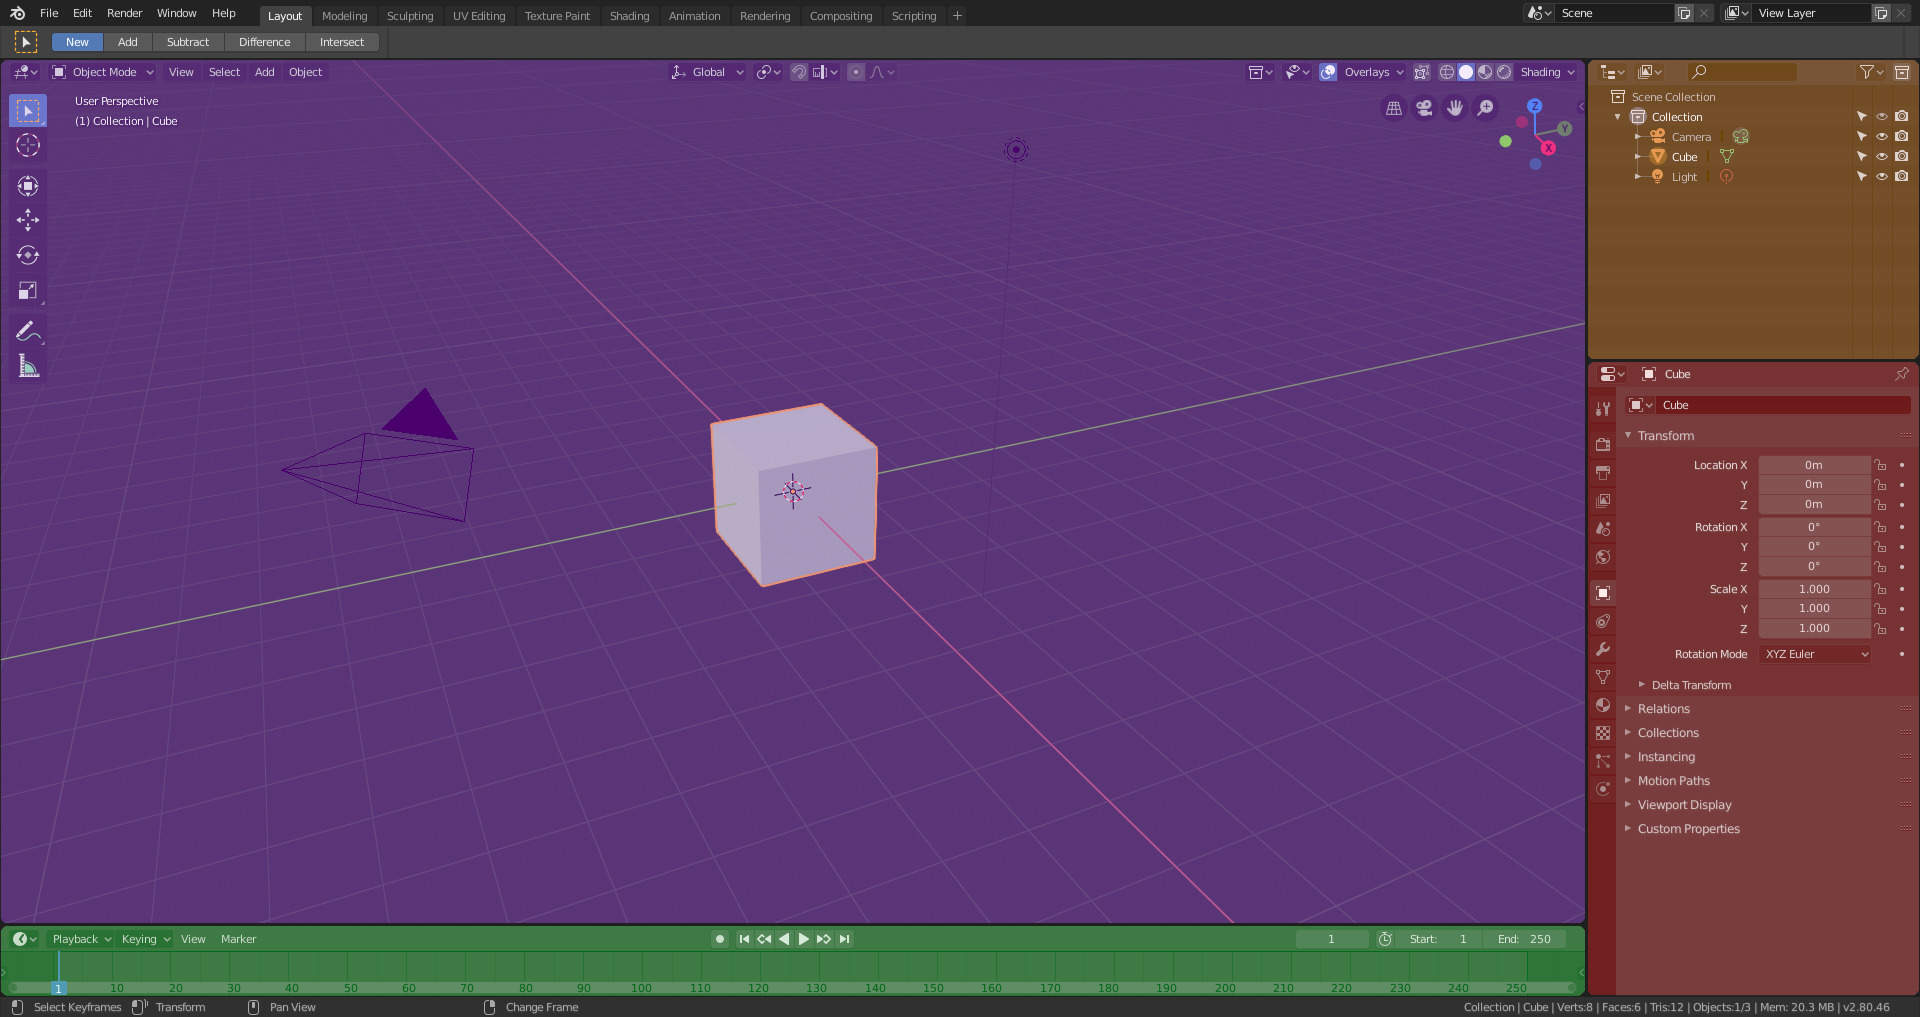
\includegraphics[scale=0.25]{UI/UI-2.png}
		\caption{Po spuštění (obarvené)}
		\label{pic:startup-2}
	\end{figure}

	Sledujme nyní obrázek \ref{pic:startup-2}. Modře je zaznačeno takzvané 3D zobrazovací
	okno, ve kterém budete pravděpodobně trávit nejvíce času. Zeleně je
	zvýrazněna Ćasová osa, která se používá hlavně při animacích. Napravo
	je červeně většina nastavení. Žlutě je Seznam objektů a skupin. Nakonec
	vršek lemuje informační panel, který obsahuje většinu ukládání, otvírání
	souborů a také se zde zobrazují procesy na pozadí jako vykreslování
	a fyzikální simulace.
	
	\paragraph{Pohyb s okny} Pokud najedete myší mezi dvě okna změní se Vám
	kurzor a můžete měnit jejich velikosti. Najetím na roh okna, kde se vám
	kurzor změní na kříž, je možné okna zavřít nebo otevřít.
	
	Obsah okna lze změnit v malém menu obsaženém v každém z oken. Na
	začátku jsou nejlépe vidět dva v obou rozích levé strany programu.
	Poznají se podle obrázku, vedle nějž se nachází šipka dolů. Po kliknutí na
	toto menu se Vám otevře výběr všech druhů oken, které si nyní
	projdeme.
	
	\begin{figure}[h]
		\centering
		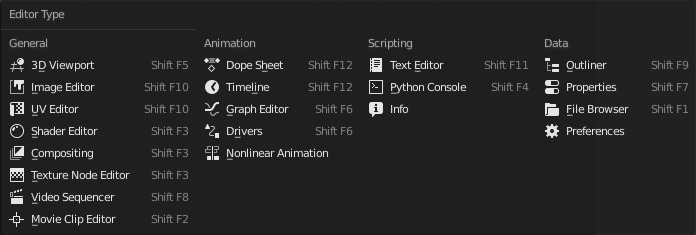
\includegraphics[scale=2]{UI/UI-WINDOWS.png}
		\caption{Výběr oken}
		\label{pic:windows-selection}
	\end{figure}

	\section{3D Zobrazení}
	
	Zde budou Vaše oči trávit nejvíce času. Okno 3D zobrazení Vám zobrazuje
celou scénu. Můžete v něm nejjednodušeji přepínat mezi objekty,
modelovat je, pohybovat a točit s nimi. Také se Vám zde promítnou
veškeré změny z jiných oken. Dále v něm můžete nahlížet do kamer
a vidíte v něm, jak vypadá Vaše scéna.
K pohybu v 3D zobrazení slouží nejlépe numpad. Klávesy 4, 8, 6 a 2 otáčí
	kameru kolem aktuálního středu. Stejný pohyb je dosažitelný přidržením
kolečka myši. 1, 7 a 3 nastaví pohled dle globálních os - přesně na pohled
shora, ze strany nebo zepředu. 9 invertuje pohled o 180 stupňů, takže pohled
zepředu otočí na pohled zezadu. K přiblížení a oddálení pohledu slouží
Klávesy [$+$] a [$-$] nebo kolečko myši.
Klávesa [Shift] změní 4 a 6 na klávesy otáčející pohled ze strany na
stranu, jako byste nakláněli hlavu. [Ctrl] změní všechny směrové klávesy
tak, aby posouvaly pohled ze strany na stranu, bez rotace.
	
	\subsection{Módy}
	Uvnitř tohoto okna se nalézá několik módů. Nejdůležitější z nichž jsou
	objektový a editační. Tyto dvě možnosti máme oddělené a přepínáme
	mezi nimi stisknutím klávesy [Tab]. Další módy jsou přístupné z menu
	v levém horním rohu.
	
	\subsection{Objektový}
	Tento mód slouží především k pohybu objektů a jako mezikrok k dalším
	módům a oknům. V objektovém módu můžete libovolně zvolit kterýkoliv
	objekt, který poté v dalších módech a oknech budete editovat, protoževšechny ostatní módy vždy pracují pouze s tímto jedním zvoleným
objektem.
	Objekt zvolíte stisknutím levého tlačítka myši kdekoli na něm.
	Pokud chcete zvolit více objektů najednou, přidržte k jejich volbě [Shift].
	
	\begin{figure}[h]
		\centering
		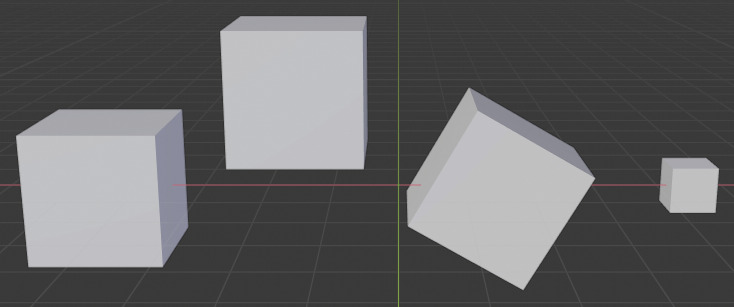
\includegraphics[scale=0.75]{UI/Translated-Cube.png}
		\caption{Transformovaná Kostka (translace, rotace, škálování)}
		\label{pic:cube-positioning}
	\end{figure}

	\paragraph{Zvolení objektů} Žlutým okrajem je zvýrazněn zvolený objekt. Ten je
	zobrazován a upravován v ostatních oknech. Oranžově jsou zvýrazněny
	další zvolené objekty, na které se také budou aplikovat translace nebo
	seskupování či další hromadné úpravy. Hlavním zvoleným objektem je
	vždy objekt, který byl do výběru přídán jako poslední. Blender referuje ke
	všem zvoleným objektům jako Selected a k hlavnímu zvolenému objektu
	jako active. Klávesou [,] zacentrujete pohled na zvolené objekty.
	
	\begin{figure}[h]
		\centering
		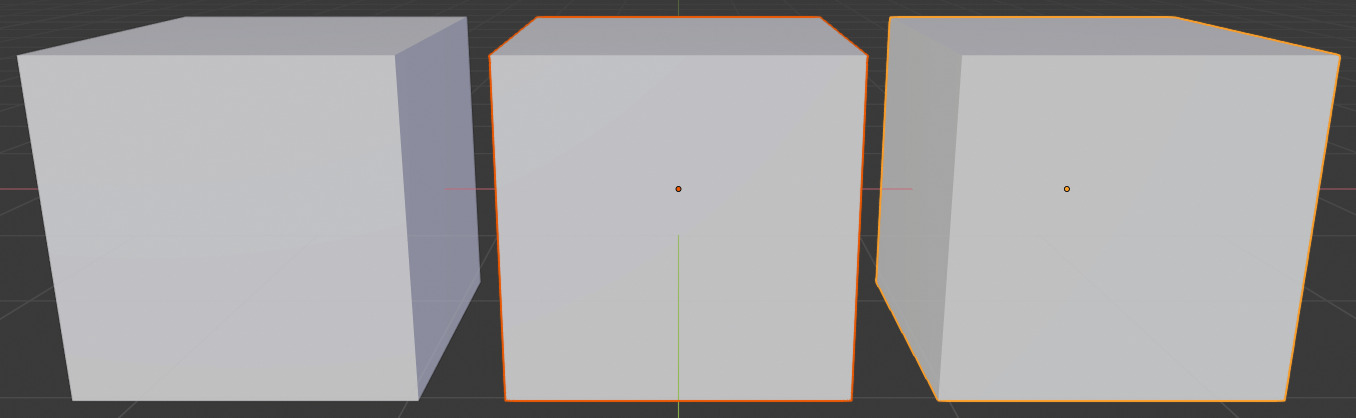
\includegraphics[scale=0.4]{UI/Selected-Cube.png}
		\caption{Volba objektů}
		\label{pic:cube-selection}
	\end{figure}

	\paragraph{Pohyb} Zde se rovnou hodí zmínit o klávesových zkratkách, těch má
Blender nespočetně, ale nyní jich budeme využívat jen několik. Nebojte,
bude to jednoduché.
	\newline \newline

	\begin{tabular}{cc}
		G & translace \\
		R & rotace \\
		S & rozměr
	\end{tabular}
	
	Poté, co jste zvolili, co chcete s objektem dělat, můžete říct přímo
	ve kterém směru. Tím, že stisknete jednu klávesu korespondující k jedné
	z os [X, Y, Z], změna se bude projevovat pouze na té ose. Pokud
	stisknete klávesu ještě jednou, tak zvolíte lokální osu namísto
	globální. Další stisknutí osu opět odemkne.
	Jsou tři osy pohybu - podle toho, k čemu jsou tyto osy kolmé, je dělíme
	především na lokální a globální. Lokální osa zahrnuje předešlé změny.
	Například krychle zobrazena níže má lokální osu X o 45 stupňů
	odkloněnou od globální osy X. Globální jsou totiž stacionární a vždy
	zůstávají stejné, osy X a Y jsou rovnoběžné s čárami zaznačenými kolem
	objektů, osa Z je na obě kolmá.
	Pokud chcete změnu provést o specifickou hodnotu, můžete ji napsat na
	klávesnici. Všechny změny se potvrzují levým tlačítkem myši a ruší se
	pravým.
\bibliography{Bibliography}
\bibliographystyle{apalike}	

\end{document}